\documentclass[10pt]{article}
\usepackage{tikz}
\usepackage[margin=0cm]{geometry}
\pagestyle{empty}

\begin{document}

\vspace*{\fill}
\begin{center}
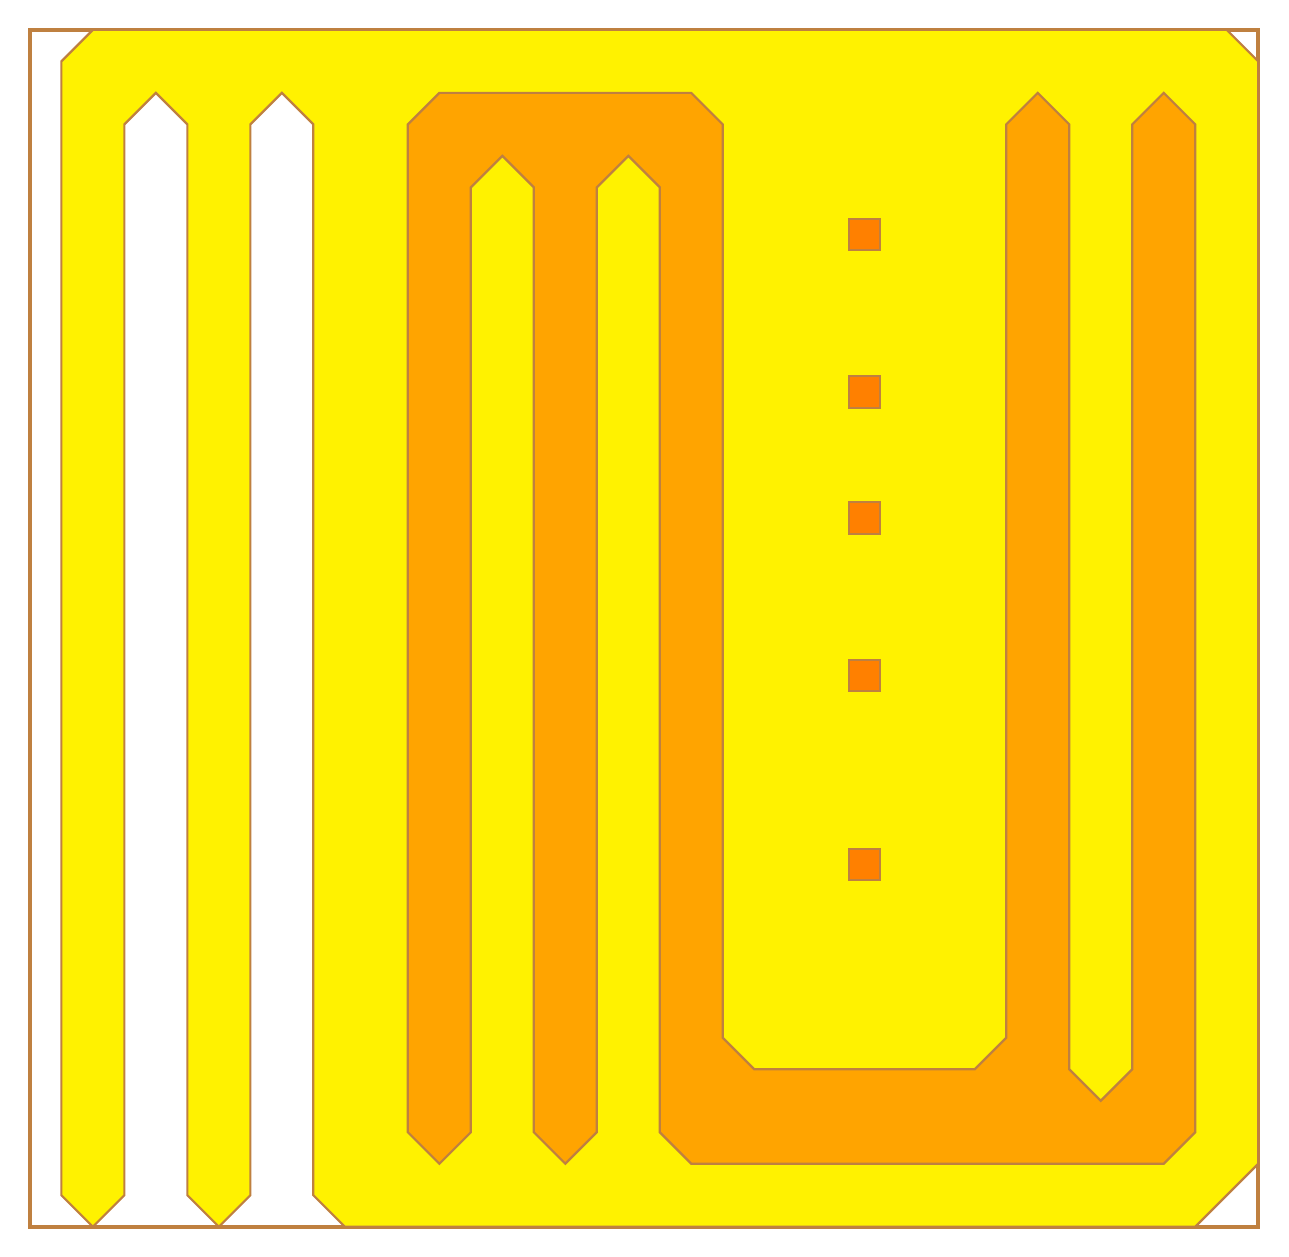
\begin{tikzpicture}[x=0.4cm, y=-0.4cm, thick, brown]
\draw[ultra thick] (0, 0) -- (39, 0) -- (39, 38) -- (0, 38) -- cycle;
%Depth 0
\filldraw[fill=orange!0!yellow] (2, 0) -- (38, 0) -- (39, 1) -- (39, 36) -- (37, 38) -- (10, 38) -- (9, 37) -- (9, 3) -- (8, 2) -- (7, 3) -- (7, 37) -- (6, 38) -- (5, 37) -- (5, 3) -- (4, 2) -- (3, 3) -- (3, 37) -- (2, 38) -- (1, 37) -- (1, 1) -- cycle;
%Depth 1
\filldraw[fill=orange!71!yellow] (13, 2) -- (21, 2) -- (22, 3) -- (22, 32) -- (23, 33) -- (30, 33) -- (31, 32) -- (31, 3) -- (32, 2) -- (33, 3) -- (33, 33) -- (34, 34) -- (35, 33) -- (35, 3) -- (36, 2) -- (37, 3) -- (37, 35) -- (36, 36) -- (21, 36) -- (20, 35) -- (20, 5) -- (19, 4) -- (18, 5) -- (18, 35) -- (17, 36) -- (16, 35) -- (16, 5) -- (15, 4) -- (14, 5) -- (14, 35) -- (13, 36) -- (12, 35) -- (12, 3) -- cycle;
\filldraw[fill=orange!100!yellow] (26, 6) -- (27, 6) -- (27, 7) -- (26, 7) -- cycle;
\filldraw[fill=orange!100!yellow] (26, 11) -- (27, 11) -- (27, 12) -- (26, 12) -- cycle;
\filldraw[fill=orange!100!yellow] (26, 15) -- (27, 15) -- (27, 16) -- (26, 16) -- cycle;
\filldraw[fill=orange!100!yellow] (26, 20) -- (27, 20) -- (27, 21) -- (26, 21) -- cycle;
\filldraw[fill=orange!100!yellow] (26, 26) -- (27, 26) -- (27, 27) -- (26, 27) -- cycle;
\end{tikzpicture}
\end{center}
\vspace*{\fill}

\end{document}
